\documentclass[pageno]{jpaper}

%replace XXX with the submission number you are given from the ISCA submission site.
\newcommand{\IWreport}{2012}

\usepackage[normalem]{ulem}
\setlength{\parskip}{\baselineskip}%
\setlength{\parindent}{0pt}%

\begin{document}

\title{3D Model Generation of Large Objects Using Autonomous Quadcopters}
\author{Edward Kelley \\
        Advisor: Szymon Rusinkiewicz
}

\date{}
\maketitle

\thispagestyle{empty}

% \begin{abstract}
% Presented is a system for
% \end{abstract}

\section{Introduction}

\subsection{Background}

%How to write the introduction?
For applications ranging from developing video games to preserving archaeological artifacts, capturing 3D models of real-world objects has become a very important task. Several different techniques for acquiring models have been developed, such as the use of laser scanners and multi-view stereo.

\subsubsection{Laser Scanners}
Laser rangefinder technology is the ``gold standard'' of 3D model acquisition in terms of quality. Modern scanners can produce sub millimeter accuracy, which make them a great choice for detailed digitization of statues. Combined with high-resolution photograph texture-mapping, very few techniques can match the precision and quality of these scans. The Digital Michelangelo Project showed the power and precision of laser scanners by scanning several different statues, including Michelangelo's David, to 1/4mm accuracy.\cite{Levoy}

\begin{figure}
\centering
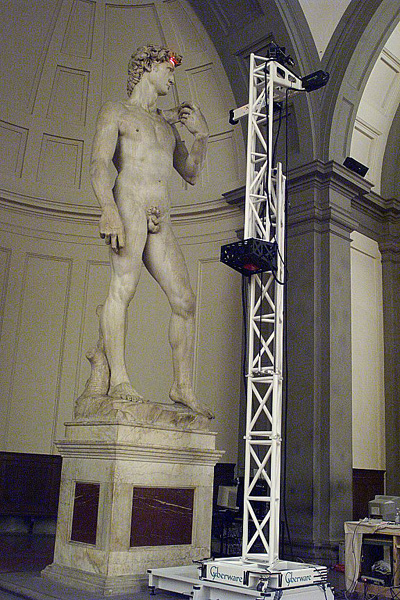
\includegraphics[height=200px]{../images/david_scan.jpg}
\caption{An example of a laser scanner setup used by the Digital Michelangelo Project \cite{Levoy}.}
\end{figure}

However, laser scanners do have several drawbacks. The equipment is extremely expensive, bulky, and fragile. The Michelangelo Project had to transport over 4 tons of equipment to Italy in order to produce their scans. Additionally, laser scans involve immense setup and can take many hours. The scan of David took over a thousand man-hours to scan and even more than that in post processing \cite{Levoy}.

%What about those hand-held scanners used for accident reconstruction

%What is the difference between photogrammetry and multi-view stereo
\subsubsection{Multi-View Stereo}
Multi-view stereo uses a collection of 2D images to reconstruct a 3D object model. By viewing a single object from hundreds of different camera positions, a 3D model can be generated. Although this technique originally required precisely known camera coordinates, recent algorithms can produce a 3D model from an unordered collection of images with unknown camera positions, assuming that there is sufficient coverage. Existing software packages such as Bundler and Agisoft Photoscan can produce high-quality 3D reconstructions using these unordered image collections. \cite{bundler}\cite{photoscan}

The ability to use a collection of images without precise camera position information means that these 3D objects can be modeled substantially faster than with a laser scanner. With a smaller object, it is a relatively simple process to take pictures of the object from many different angles. However, for a larger object, such as a statue or building, the problem of gathering imagery becomes substantially more difficult.

\begin{figure}
\centering
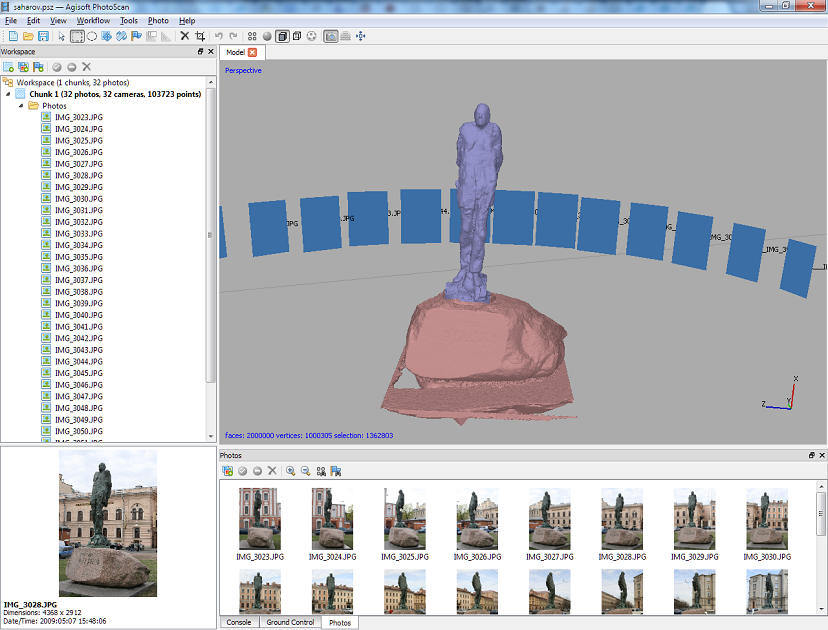
\includegraphics[height=200px]{../images/photoscan.png}
\caption{A 3D model of a statue generated by Agisoft Photoscan. Notice the derived camera planes encompassing the statue \cite{photoscan}.}
\end{figure}

\subsection{Problem Definition}
We look to create a system to capture imagery of large 3D objects for use in multi-view stereo software. This system has several requirements.

\begin{enumerate}
\item
\textbf{Low Cost}

The system should be substantially cheaper than laser scanning.

\item
\textbf{Easy to Use}

This system should be able to be deployed by users with minimal training. Additionally, the hardware should be off-the-shelf and easily accessible.

\item
\textbf{Complete Coverage}

The system must be able to capture images from a wide variety of positions, completely covering every part of the target object.

\item
\textbf{High Quality Imagery}

The system must produce sufficiently high resolution, non-blurry images for use in multi-view stereo software.

\end{enumerate}

\subsection{Proposed Solution}

We propose using low-cost autonomous quadcopters to gather imagery needed for use in multi-view stereo software. By flying a quadcopter with a mounted camera around the target object, we can quickly and thoroughly capture images of the target from a wide variety of positions. Using quadcopters has many advantages.

\begin{enumerate}
\item
Quadcopters can capture images from positions unreachable by ground-based cameras.

\item
By methodically flying around the target object at different altitudes, we can guarantee complete coverage of the target object.

\item
The imagery can be captured very quickly, on the order of a few minutes.

\item
Quadcopters are small, portable, and easily deployable.


\end{enumerate}

\subsection{Hardware}
For this project, we are using the Parrot AR.Drone 2.0. Although originally designed as a high-tech toy, many have found the AR.Drone to be a useful platform for research. At only around \$300, the AR.Drone is substantially less expensive than most quadcopters which typically cost a couple thousand dollars. However, despite the low cost, the AR.Drone boasts an impressive array of sensors and technology.

The drone has two cameras, one forward-facing 720p wide-angle, and one downward-facing QVGA camera. The drone has an on-board processor to automatically stabilize itself using its gyroscope, accelerometer, and magnetometer readings. Additionally, the drone has both ultrasound and pressure sensors for altitude measurement.

\begin{figure}
\centering
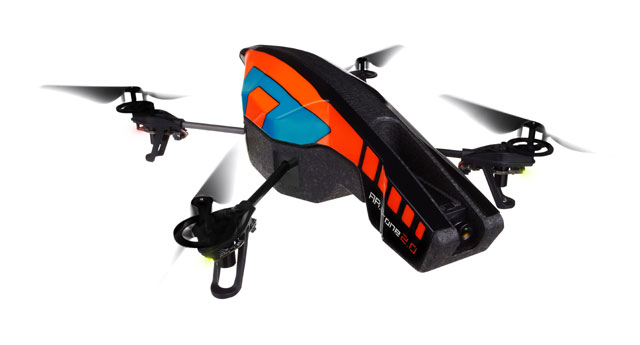
\includegraphics[height=200px]{../images/drone_in.jpg}
\caption{The Parrot AR.Drone 2.0 with Indoor Hull}
\end{figure}

\subsection{Related Work}

The past decade has seen a huge increase in the use of quadcopters for a variety of applications. With the improvement of stabilization software, quadcopters have seen a rise in popularity as a stable, cheap, and highly maneuverable aerial platform. 

TODO: WRITE RELATED WORK


\section{Project Status}

\subsection{Quadcopter Interface}

After doing substantial research, we decided on using  ``ardrone\_autonomy'' a Robot Operating System (ROS) driver for the AR.Drone. This package allows us to easily subscribe to the navdata from the drone as well as publish commands. ROS provides a nice framework for organizing different elements of our system as well as integration with libraries such as OpenCV.

\subsection{Software}

Our first step was to build a ROS package that would allow us to issue basic commands to the drone and receive video. We built a graphical user interface so that we could easily control the drone manually. We then worked on using the OpenCV library with the video feed. Currently, we can track detected features between frames, which will be important for estimating object coverage. We have also started to work on the problem of localization. We built a particle filter that will propagate a position estimate of the drone based on the velocity readings from the drone.

\subsection{Next Steps}

After testing the drone with basic commands, we realized that localization will be a major issue. Using only the dead reckoning velocity measurements of the drone, the position estimate becomes very inaccurate after only a few instructions. Therefore, we are going to look into using visual tags on the ground along the bounding box of the flight path. We can use the computed relative position to these tags to greatly increase the accuracy of our position estimate. Additionally, these may help us compensate for some of the wind drift we have been experiencing. After producing a more reliable position estimate, we can work on motion planning and coverage estimation.

\subsection{Timeline}

\textbf{2/18/13} Determine relative position to visual tags.

\textbf{2/25/13} Localization correction using visual tags.

\textbf{3/11/13} Fly programmed pattern around a statue.

\textbf{3/25/13} Create voxel representation of explored/unexplored space.

\textbf{4/1/13} Test system on different objects. Start writing report.

\textbf{4/22/13} Full rough draft of final report.

\textbf{5/6/13} Final draft turned in.



%What does this do?
% \bstctlcite{bstctl:etal, bstctl:nodash, bstctl:simpurl}

\newpage
\bibliographystyle{IEEEtranS}
\bibliography{../Bibliography/sources}
\nocite{*}

\end{document}

